\documentclass{article}

\usepackage[margin=.75in]{geometry}
\usepackage{listings}
\usepackage{amsmath}
\usepackage[hidelinks]{hyperref}
\usepackage{graphicx}

\lstset{
    basicstyle=\ttfamily,
    mathescape
}

\author{Damien Prieur}
\title{Homework 4 \\ CS 457}
\date{}

\begin{document}

\maketitle

\section*{Question 1}
You are given a red-black tree $T$ with 15 internal nodes (nodes that hold key values)
that form a \emph{full} binary tree of height 3 (i.e., a full binary tree of height 4 if you include
the NIL leaves). Can you assign colors to the nodes so that a call to \textsc{RB-Insert}($T,z$) for
\emph{any} new key value $z.key$ will cause \textsc{RB-Insert-Fixup}($T,z$) to change the color of the
root to red before switching it back to black? The initial assignment of colors needs to obey the
red-black properties. If such a color assignment exists, then provide a sequence of 15 numbers whose
insertion (in that order) would lead to such a tree, along with a figure of the resulting tree. If not,
then explain why such an assignment cannot exist, using the fact that the tree needs to satisfy the
red-black properties. You can use the applet \url{https://www.cs.usfca.edu/~galles/visualization/RedBlack.html}
and read through Chapter 13 from your textbook if you would like to better understand how red-black trees work.

\begin{figure}[h]
    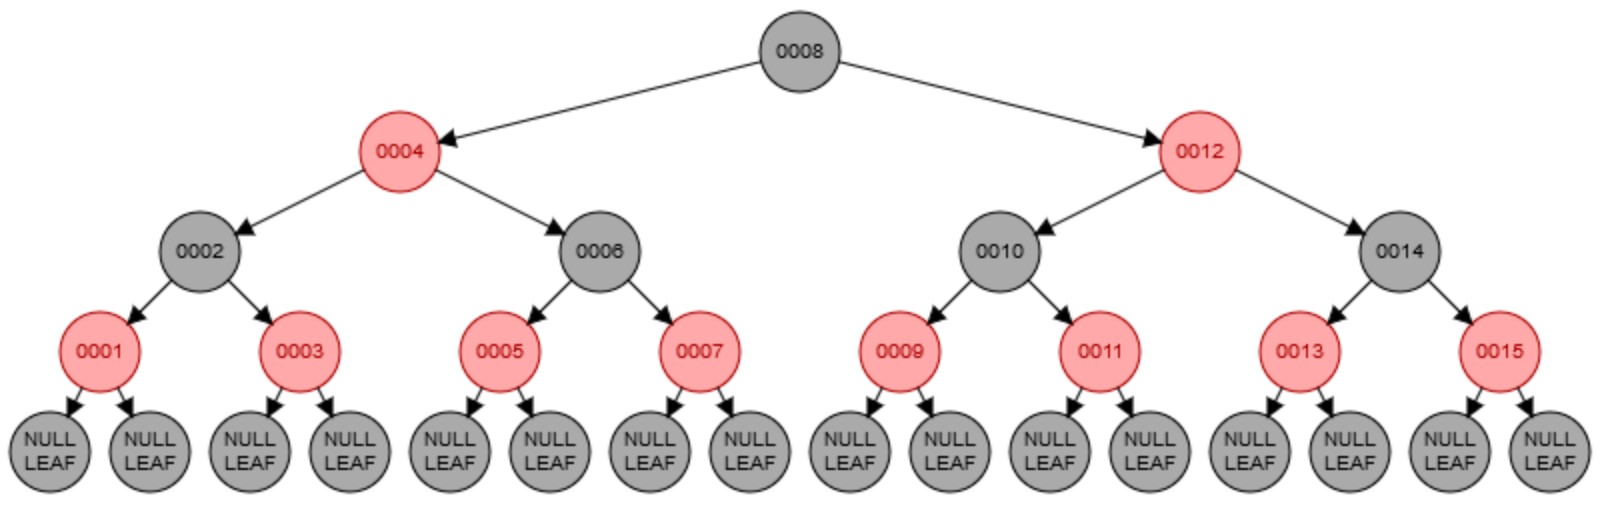
\includegraphics[width=\linewidth]{full_RB_tree.jpg}
\end{figure}

Insertion order:
8,4,12,2,14,6,10,1,3,5,7,9,11,13,15

\section*{Question 2}
A full $k$-ary tree is a (rooted) tree whose nodes either have exactly $k$ children
(internal nodes) or have no children (leaves). \emph{Using induction}, formally prove that every full
$k$-ary tree that has $x$ internal nodes has exactly $kx+1$ nodes in total. Note that for full
\emph{binary} trees, i.e., when $k=2$, this would imply that the total number of nodes is $2x+1$,
which would verify what Cameron suggested in class (that the total number of nodes of full binary
trees is always odd).
\\
\\
For the base case we can look at a tree with one node. This tree has $0$ internal nodes so we have $k\cdot 0 + 1=1$ node in our tree.
\\
For our inductive step we can look at how we can add nodes to increase our internal node count.
We can select any leaf, we can't choose an internal node to add nodes to as they would become over-populated.
With the leaf we must add k leaves so that our tree is still complete.
Doing so causes our chosen leaf to become an internal node and adds k new nodes.
\\
Assume that any $k$-ary tree that has $n$ internal nodes has exactly $kx+1$ nodes in total.
To show that this holds for $n+1$ internal nodes we begin with our assumption for n.
$$Total \; nodes = kn+1$$
Based on the argument above selecting a leaf to add new nodes to increases our internal node count by $1$, $n'=n+1$, and increases our total node count by $k$, $Total \; nodes'=kn+1+k$.
Rearranging these terms we get
$$Total \; nodes' = k(n+1)+1 = kn'+1$$
Which agrees with our original equation for n+1.


\section*{Question 3}
Using proof by induction, show that there are at most $\lceil n/2^{h+1}\rceil$
nodes of height $h$ in any $n$-element heap. Make sure to clearly state your base case and your
inductive step arguments. Also note that you need to prove the aforementioned upper bound for the
number of nodes of height $h$ for \emph{every} value of $n$ and \emph{every} $n$-element heap.

Heaps - nearly complete binary tree except for, possibly, the lowest level


\section*{Question 4}
You start a new tech business and you reach the point where you have offices both in the
east coast and in the west coast. There are different operating costs involved in running your business
in each location, so you may need to move back and forth across the coasts in order to minimize the total
costs. However, there are moving costs involved in traveling from one coast to the other which complicate
your problem. More formally, for each month $i=1,\dots, n$ you have an operating cost $e_i$ associated
with running your business in the east coast during that month and an operating cost $w_i$ for the west coast.
You can begin working in either coast, but after any subsequent travel from one coast to another you suffer
a fixed travel cost of $c$. Given input $\{e_1,\dots, e_n\}$, $\{w_1,\dots, w_n\}$, and $c$, provide a $O(n)$
time algorithm that outputs a plan defining which coast you will work from each month, and minimizes your
total cost (operating costs plus travel costs).

For example, if the number of months was $n=5$, a possible plan could be to work from the east coast during
the first two months, then spend the next two months working from the west coast, and return to the east coast
for the fifth and final month. The total cost in this case would be $e_1+e_2+c+ w_3+w_4+c +e_5$, where the
two costs of $c$ are due to the change of coast. Provide detailed pseudocode for your proposed algorithm, as
well as an explanation regarding why it works and why its running time is indeed $O(n)$.

For each month keep track of the best way to get to that coast for that month.
\\
We find the solution by solving two subproblems, one for the best way to end on the east coast for month i, and the other being the same but for the west coast., one for the best way to end on the east coast for month i, and the other being the same but for the west coast.





\section*{Question 5}
You are planning to attend a music and arts festival that hosts multiple events that
you are interested in, but many of these events may (partially) overlap. Assume that you get some value
$v_i$ from attending an event $i$, but you get this value only if you are there for the whole duration
of the event; you get no value if you have to miss part of it. Given such a set of events, $E$, your
goal is to choose a non-overlapping set of events, $E'\subseteq E$, to attend, aiming to maximize your
total value. More formally, for each event $i\in E$ you have a start time $s_i$ and a finish time $f_i$ and
you want to design an algorithm that runs in time $O(n\log n)$, where $n$ is the total number of events,
and the output of the algorithm is a set $E'\subseteq E$ such that for any two events $i,j\in E'$ we have
$f_i\leq s_j$ or $f_j \leq s_i$ (no overlap) and the total value $\sum_{i\in E'} v_i$ is maximized. Provide
detailed pseudocode for your proposed algorithm (you can use sorting as a subroutine), as well as an explanation
regarding why it works and why its running time is indeed $O(n\log n)$.

sort by start times, then basically apply the same algorithm as in question 4.

\end{document}
